\subsection{\Camelyon}\label{sec:app_camelyon}
Models for medical applications are often trained on data from a small number of hospitals, but with the goal of being deployed more generally across other hospitals.
However, variations in data collection and processing can degrade model accuracy on data from new hospital deployments \citep{zech2018radio,albadawy2018tumor}.
In histopathology applications---studying tissue slides under a microscope---this variation can arise from sources like differences in the patient population or in slide staining and image acquisition \citep{veta2016mitosis,komura2018machine,tellez2019quantifying}.

We study this shift on a patch-based variant of the Camelyon17 dataset \citep{bandi2018detection}.

\subsubsection{Setup}
\paragraph{Problem setting.}
We consider the domain generalization setting, where the domains are hospitals, and our goal is to learn models that generalize to data from a hospital that is not in the training set (\reffig{dataset_camelyon}).
The task is to predict if a given region of tissue contains any tumor tissue,
which we model as binary classification.
Concretely, the input $x$ is a 96x96 histopathological image, the label $y$ is a binary indicator of whether the central 32x32 region contains any tumor tissue, and the domain $d$ is an integer that identifies the hospital that the patch was taken from.

\paragraph{Data.}
The dataset comprises 450,000 patches extracted from 50 whole-slide images (WSIs) of breast cancer metastases in lymph node sections, with 10 WSIs from each of 5 hospitals in the Netherlands.
Each WSI was manually annotated with tumor regions by pathologists, and the resulting segmentation masks were used to determine the labels for each patch.
We also provide metadata on which slide (WSI) each patch was taken from, though our baseline algorithms do not use this metadata.

We split the dataset by domain (i.e., which hospital the patches were taken from):
\begin{enumerate}
  \item \textbf{Training:} 302,436 patches taken from 30 WSIs, with 10 WSIs from each of the 3 hospitals in the training set.
  \item \textbf{Validation (OOD):} 34,904 patches taken from 10 WSIs from the 4th hospital. These WSIs are distinct from those in the other splits.
  \item \textbf{Test (OOD):} 85,054 patches taken from 10 WSIs from the 5th hospital, which was chosen because its patches were the most visually distinctive. These WSIs are also distinct from those in the other splits.
  \item \textbf{Validation (ID):} 33,560 patches taken from the same 30 WSIs from the training hospitals.
\end{enumerate}
We do not provide a Test (ID) set, as there is no practical setting in which we would have labels on a uniformly randomly sampled set of patches from a WSI, but no labels on the other patches from the same WSI.


\paragraph{Evaluation.}
We evaluate models by their average test accuracy across patches. Histopathology datasets can be unwieldy for ML models, as individual images can be several gigabytes large; extracting patches involves many design choices; the classes are typically very unbalanced; and evaluation often relies on more complex slide-level measures such as the free-response receiver operating characteristic (FROC) \citep{gurcan2009histopathological}.
To improve accessibility, we pre-process the slides into patches and balance the dataset so that each split has a 50/50 class balance, making average accuracy is a reasonable measure of performance \citep{veeling2018rotation, tellez2019quantifying}.

\paragraph{Potential leverage.}
Prior work has shown that differences in staining between hospitals are the primary source of variation in this dataset, and that specialized stain augmentation methods can close the in- and out-of-distribution accuracy gap on a variant of the dataset based on the same underlying slides \citep{tellez2019quantifying}.
However, the general task of learning histopathological models that are robust to variation across hospitals (from staining and other sources) is still an open research question.
In this way, the \Camelyon dataset is a controlled testbed for general-purpose methods that can learn to be robust to stain variation between hospitals, given a training set from multiple hospitals.


\subsubsection{Baseline results}

\begin{table*}[!t]
  \caption{Baseline results on \Camelyon. In-distribution (ID) results correspond to the train-to-train setting. Parentheses show standard deviation across 10 replicates. Note that the standard error of the mean is smaller (by a factor of $\sqrt{10}$).
  }
  \label{tab:results_camelyon}
  \centering
  \begin{tabular}{lcccc}
  \toprule
  Algorithm & Validation (ID) accuracy & Validation (OOD) accuracy & Test (OOD) accuracy\\
  \midrule
  ERM        & 93.2 (5.2) & 84.9 (3.1) & \textbf{70.3} (6.4)\\
  CORAL      & 95.4 (3.6) & 86.2 (1.4) & 59.5 (7.7)\\
  IRM        & 91.6 (7.7) & 86.2 (1.4) & 64.2 (8.1)\\
  Group DRO  & 93.7 (5.2) & 85.5 (2.2) & 68.4 (7.3)\\
  \bottomrule
  \end{tabular}
\end{table*}

\begin{table*}[!t]
  \caption{Mixed-to-test comparison for ERM models on \Camelyon.
  In the official OOD setting, we train on data from three hospitals and evaluate on a different test hospital, whereas in the mixed-to-test ID setting,
  we add data from one extra slide from the test hospital to the training set.
  The official Test (OOD) set has data from 10 slides, but for this comparison, we report performance for both splits on the same 9 slides (without the slide that was moved to the training set).
  This makes the numbers (71.0 vs. 70.3) for the official split slightly different from \reftab{results_camelyon}.
  Parentheses show standard deviation across 10 replicates.
  Note that the standard error of the mean is smaller (by a factor of $\sqrt{10}$).
  }
  \label{tab:drop_camelyon}
  \centering
  \begin{tabular}{lcccc}
  \toprule
  Setting                                       & Algorithm & Test (OOD) accuracy\\
  \midrule
  Official      (train on ID examples)        & ERM       & 71.0 (6.3)\\
  Mixed-to-test (train on ID + OOD examples)  & ERM       & \textbf{82.9} (9.8)\\
  \bottomrule
  \end{tabular}
\end{table*}

\paragraph{Model.}
For all experiments, we use DenseNet-121 models \citep{huang2017densely} models trained from scratch on the 96 $\times$ 96 patches, following prior work \citep{veeling2018rotation}. These models used a learning rate of $10^{-3}$, $L_2$-regularization strength of $10^{-2}$, a batch size of 32, and SGD with momentum (set to 0.9), trained for 5 epochs with early stopping.
We selected hyperparameters by a grid search over learning rates $\{10^{-4}$, $10^{-3}$, $10^{-2}\}$, and $L_2$-regularization strengths $\{0, 10^{-3}, 10^{-2}\} $.
We report results aggregated over 10 random seeds.

\paragraph{ERM results and performance drops.}
\reftab{results_camelyon} shows that the model was consistently accurate on the train-to-train in-distribution (ID) validation set and to a lesser extent on the out-of-distribution (OOD) validation set, which was from a held-out hospital.
However, it was wildly inconsistent on the test set, which was from a different held-out hospital,
with a standard deviation of 6.4\% in accuracies across 10 random seeds.
There is a large gap between train-to-train ID validation and OOD validation accuracy, and between OOD validation and OOD test accuracy (in part because we early stop on the highest OOD validation accuracy).
Nevertheless, we found that using the OOD validation set gave better results than using the ID validation set; see \refapp{experiments_id_vs_ood} for more discussion.

We ran an additional mixed-to-test comparison, where we moved 1 of the 10 slides\footnote{This slide was randomly chosen and corresponded to about 6\% of the test patches; some slides contribute more patches than others because they contain larger tumor regions.} from the test hospital to the training set and tested on the patches from the remaining 9 slides.
The mixed-to-test setting gives significantly higher accuracy on the reduced test set (\reftab{drop_camelyon}), suggesting that the observed performance drop is due to the distribution shift, as opposed to the intrinsic difficulty of the examples from the test hospital.
We note that this mixed-to-test comparison mixes in only a small amount of test data and is therefore likely to be an underestimate of in-distribution performance on the test set; we opted to only mix in 1 slide so as to preserve enough test examples to be able to accurately estimate model performance.

\paragraph{Additional baseline methods.}
We trained models with CORAL, IRM, and Group DRO, treating each hospital as a domain.
However, they performed comparably or worse than the ERM baseline.
For the CORAL and IRM models, our grid search selected the lowest values of their penalty weights (0.1 and 1, respectively) based on OOD validation accuracy.


\begin{figure}[t]
  \centering
  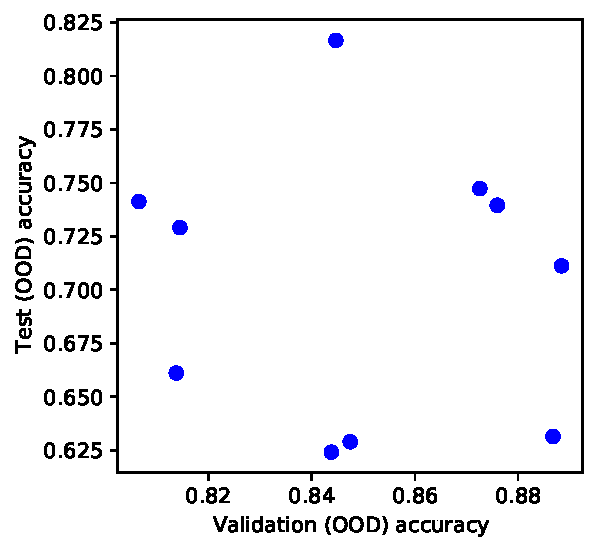
\includegraphics[width=0.4\linewidth]{figures/camelyon_seeds.pdf}
  \caption{
    Test (OOD) accuracy versus validation (OOD) accuracy for different random seeds on \Camelyon, using the same hyperparameters. The test accuracy is far more variable than the validation accuracy (note the differences in the axes), in part because we early stop on the highest OOD validation accuracy.
  }
  \label{fig:seeds_camelyon}
\end{figure}


\paragraph{Discussion.}
These results demonstrate a subtle failure mode when considering out-of-distribution accuracy: there are models (i.e., choices of hyperparameters and random seeds) that do well both in- and out-of-distribution, but we cannot reliably choose these models from just the training/validation set.
Due to the substantial variability in test accuracy on \Camelyon (see \reffig{seeds_camelyon}), we ask researchers to submit leaderboard submissions with results from 10 random seeds, instead of the 3 random seeds required for other datasets.

Many specialized methods have been developed to handle stain variation in the context of digital histopathology. These typically fall into one of two categories: data augmentation methods that perturb the colors in the training images (e.g., \citet{liu2017detecting,bug2017context,tellez2018whole})
or stain normalization methods that seek to standardize colors across training images (e.g., \citet{macenko2009method,bentaieb2017adversarial}).
These methods are reasonably effective at mitigating stain variation, at least in some contexts \citep{tellez2019quantifying,miller2021line}, though the general problem of learning digital histopathology models that can be effectively deployed across multiple hospitals/sites is still an open challenge.

To facilitate more controlled experiments, we will have two leaderboard tracks for \Camelyon.
For the first track, which focuses on general-purpose algorithms, submissions should not use color-specific techniques (e.g., color augmentation) and should also train their models from scratch, instead of fine-tuning models that are pre-trained from ImageNet or other datasets.
For the second track, submissions can use any of those techniques, including specialized methods for dealing with stain variation.
These separate tracks will help to disentangle the contributions of more general-purpose learning algorithms and model architectures from the contributions of specialized augmentation techniques or additional training data.


\subsubsection{Broader context}
Other than stain variation, there are many other distribution shifts that might occur in histopathology applications. For example, patient demographics might differ from hospital to hospital: some hospitals might tend to see patients who are older or more sick, and patients from different backgrounds and countries vary in terms of cancer susceptibility \citep{henderson2012influence}.
Some cancer subtypes and tissues of origin are also more common than others, leading to potential subpopulation shift issues, e.g,. a rare cancer subtype in one context might be more common in another; or even if it remains rare, we would seek to leverage the greater quantity of data from other subtypes to improve model accuracy on the rare subtype \citep{weinstein2013cancer}.

Beyond histopathology, variation between different hospitals and deployment sites has also been shown to degrade model accuracy in other medical applications such as diabetic retinopathy \citep{beede2020human} and chest radiographs \citep{zech2018radio,phillips2020chexphoto}, including recent work on COVID-19 detection \citep{degrave2020ai}.
Even within the same hospital, process variables like which scanner/technician took the image can significantly affect models \citep{badgeley2019deep}.

In these medical applications, the gold standard is to evaluate models on an independent test set collected from a different hospital (e.g., \citet{beck2011systematic,liu2017detecting,courtiol2019deep,mckinney2020international}) or at least with a different scanner within the same hospital (e.g., \citet{campanella2019clinical}).
However, this practice has not been ubiquitous due to the difficulty of obtaining data spanning multiple hospitals \citep{esteva2017dermatologist,bejnordi2017diagnostic,codella2019skin,veta2019predicting}.
The baseline results reported above show that even evaluating on a single different hospital might be insufficient, as results can vary widely between different hospitals (e.g., between the validation and test OOD datasets).
We hope that the \Camelyon dataset, which has multiple hospitals in the training set and  independent hospitals in the validation and test sets, will be useful for developing models that can generalize reliably to new hospitals and contexts \citep{chen2020ethical}.

\subsubsection{Additional details}\label{sec:app_camelyon_details}
\paragraph{Data processing.}
The \Camelyon dataset is adapted from whole-slide images (WSIs) of breast cancer metastases in lymph nodes sections, obtained from the CAMELYON17 challenge \citep{bandi2018detection}.
Each split is balanced to have an equal number of positive and negative examples.
The varying number of patches per slide and hospital is due to this class balancing, as some slides have fewer tumor (positive) patches.
We selected the test set hospital as the one whose patches were visually most distinct; the difference in test versus OOD validation performance shows that the choice of OOD hospital can significantly affect performance.

From these WSIs, we extracted patches in a standard manner, similar to \citet{veeling2018rotation}.
The WSIs were scanned at a resolution of 0.23$\mu$m--0.25$\mu$m in the original dataset, and each WSI contains multiple resolution levels, with approximately 10,000$\times$20,000 pixels at the highest resolution level
\citep{bandi2018detection}.
We used the third-highest resolution level, corresponding to reducing the size of each dimension by a factor of 4.
We then tiled each slide with overlapping 96$\times$96 pixel patches with a step size of 32 pixels in each direction (such that none of the central 32$\times$32 regions overlap), labeling them as the following:
\begin{itemize}
  \item \emph{Tumor} patches have at least one pixel of tumor tissue in the central 32$\times$32 region. We used the pathologist-annotated tumor annotations provided with the WSIs.
  \item \emph{Normal} patches have no tumor and have at least 20\% normal tissue in the central 32$\times$32 region. We used Otsu thresholding to distinguish normal tissue from background.
\end{itemize}
We discarded all patches that had no tumor and \textless20\% normal tissue in the central 32$\times$32 region.

To maintain an equal class balance, we then subsampled the extracted patches in the following way.
First, for each WSI, we kept all tumor patches unless the WSI had fewer normal than tumor patches, which was the case for a single WSI; in that case, we randomly discarded tumor patches from that WSI until the numbers of tumor and normal patches were equal.
Then, we randomly selected normal patches for inclusion such that for each hospital and split, there was an equal number of tumor and normal patches.

\paragraph{Modifications to the original dataset.}
The task in the original CAMELYON17 challenge \citep{bandi2018detection} was the patient-level classification task of determining the pathologic lymph node stage of the tumor present in all slides from a patient. In contrast, our task is a lesion-level classification task. Patient-level, slide-level, and lesion-level tasks are all common in histopathology applications.
As mentioned above, the original dataset provided WSIs and tumor annotations,
but not a standardized set of patches, which we provide here.
Moreover, it did not consider distribution shifts; both of the original training and test splits contained slides from all 5 hospitals.

The \Camelyon patch-based dataset is similar to one of the datasets used in \citet{tellez2019quantifying}, which was also derived from the CAMELYON17 challenge; there, only one hospital is used as the training set, and the other hospitals are all part of the test set.
\Camelyon is also similar to PCam \citep{veeling2018rotation}, which is a patch-based dataset based on an earlier CAMELYON16 challenge; the data there is derived from only two hospitals.

\paragraph{Additional data sources.}
The full, original CAMELYON17 dataset contains 1000 WSIs from the same 5 hospitals, although only 50 of them (which we use here) have tumor annotations. The other 950 WSIs may be used as unlabeled data. Beyond the CAMELYON17 dataset, the largest source of unlabeled WSI data is the Cancer Genome Atlas \citep{weinstein2013cancer}, which typically has patient-level annotations (e.g., patient demographics and clinical outcomes).
